\documentclass[aspectratio=169]{beamer}
\usepackage{will_handley}

% Commands
% --------
% - \arxiv{arxiv number}
% - \cols{width}{lh column}{rh column}
% -  \begin{fig(left|right)}[fractional width (e.g 0.6) ]{name of image}
%        content of other column
%    \end{fig(left|right)}

% Talk details
% ------------
\title{Review on Statistical Tools and Samplers}
\date{26\textsuperscript{th} November 2021}

\begin{document}

\begin{frame}
    \titlepage
\end{frame}

\begin{frame}
    \frametitle{The name of the game}
    \begin{itemize}
        \item Many considerations in this talk applicable to Bayesian, Frequentist or ``Monte Carlo'' 
        \item I acknowledge my Bayesian bias!
        \item In general consider a function $\mathcal{P}(\theta)$ over some $d$-dimensional space
        \item This function can be ``forward calculated'': given any location $\theta$ in space, can compute $P$
        \item Analytic pen-and-paper results assumed unavailable/impossible
        \item We wish to:
            \begin{itemize}
                \item Explore the region(s) of high $\mathcal{P}$
                \item Generate representative samples, either in this region, or in the tails
                \item find the hypervolume under the curve $\int P(\theta) d\theta$
            \end{itemize}
        \item Examples include
            \begin{itemize}
                \item Generating samples from a Bayesian posterior distribution
                \item Generating datasets for computing test statistics
                \item Generating Monte Carlo events 
                \item Computing Bayesian evidences for model comparison
                \item Computing cross sections
            \end{itemize}
    \end{itemize}
\end{frame}

\begin{frame}
    \frametitle{Notation}
    \begin{itemize}
        \item Space of parameters $\theta$
        \item Probability distribution/function $\mathcal{P}(\theta)$
        \item Region of valid parameters/support of function/prior/measure $\pi(\theta)$
            \begin{itemize}
                \item Note that for any numerical method even if not specified there is an implicit measure imposed by floating point arithmetic
            \end{itemize}
    \end{itemize}
\end{frame}

\begin{frame}
    \frametitle{Why is this hard?}
    \begin{itemize}
        \item In general, the region of significantly non-zero $\mathcal{P}$ (the typical set) is very ``small''
        \item This problem gets exponentially worse the higher the dimensionality $d$ becomes

        \item Quantify this with the Kullback-Liebler divergence between distributions $\mathcal{P}(\theta)$ and $\pi(\theta)$
    \end{itemize}
    \begin{columns}[onlytextwidth]
        \column{0.6\textwidth}
        \vspace{-5pt}
        \[
        \hspace{-15pt}
        \mathcal{D} = \int \mathcal{P}(\theta) \log\frac{\mathcal{P}(\theta)}{\pi(\theta)} d\theta \sim \log \frac{V_\pi}{V_\mathcal{P}}, \quad \frac{V_\pi}{V_\mathcal{P}} \sim {\left(\frac{\ell_\mathcal{\pi}}{\ell_\mathcal{P}}\right)}^d \]
        \vspace{-10pt}
        \begin{itemize}
            \item Note that this is \alert{not} a distance
            \item One can verify $\sim$ as being $=$ for top hat distributions over regions $R_\mathcal{P}$  and $R_\mathcal{\pi}$ with volumes $V_\mathcal{P}$ and $V_\mathcal{\pi}$ respectively:
                \[\hspace{-20pt}
                    \mathcal{P}(\theta) = \left\{
                        \begin{array}{cl}
                            1/V_\mathcal{P} & \theta \in R_\mathcal{P}\\
                            0 & \text{otherwise}\\
                        \end{array}
                    \right.
                    \quad
                    \pi(\theta) = \left\{
                        \begin{array}{cl}
                            1/V_\pi & \theta \in R_\pi\\
                            0 & \text{otherwise}\\
                        \end{array}
                    \right.
                \]
            \item The integral smooths this over the distribution $\mathcal{P}$
        \end{itemize}
        \column{0.4\textwidth}
        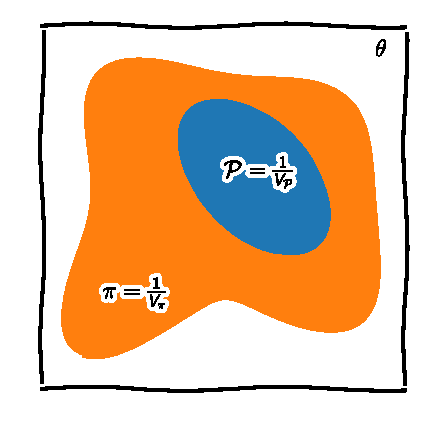
\includegraphics{figures/volumes.pdf}
    \end{columns}
\end{frame}

\begin{frame}
    \frametitle{How not to do it}
    \begin{itemize}
        \item The worst way to explore/integrate a probability distribution/generate samples is to randomly sample the space using $\pi(\theta)$~\arxiv{2012.09874}
        \item Gridding is also equivalently bad
        \item Whilst this works in low dimensions, if each parameter is confined within some fraction $f\sim\ell_\mathcal{P}/\ell_\pi$ of the space, then the volume fraction $\sim\mathcal{O}(f^d)$, or equivalently $\mathcal{D}\sim d\log f$ 
        \item Random sampling has an efficiency of $\boxed{\approx e^{-\mathcal{D}} \sim e^{-d\log f} = f^{-d}}$
        \item If you find that naive tail sampling is performant for e.g. importance sampling and unweighting, then your function likely has an unusual $\mathcal{D}$ scaling with $d$. 
        \item Turning this around, you can use the inefficiency of random sampling to estimate $\mathcal{D}$
        \item Paper being released soon:

            \hfill \emph{``Exploring phase space with Nested Sampling''} Handley, \textbf{Jan{\ss}en}, Schumann \& \textbf{Yallup}\\
            Also \textbf{Carragher} et al~\arxiv{2101.00428}
    \end{itemize}
\end{frame}

\begin{frame}
    \frametitle{Why do sampling}
    \begin{itemize}
        \item Instead of randomly sampling the space, samples $\theta\sim\mathcal{P}$ drawn from the distribution exponentially concentrate around the significantly non-zero region of $\mathcal{P}$
        \item This represents an optimal compression of the space
        \item If you have generated a set of samples drawn from a distribution $S=\{\theta_i : i=1\cdots N,\theta_i\sim\mathcal{P}\}$, then one can compute integrals
            \[ \langle f(\theta) \rangle_\mathcal{P} = \int f(\theta) \mathcal{P}(\theta) d\theta \approx \sum_{\theta_i\in S} f(\theta_i) \]
        \item Typically this is done using weighted samples $S=\{(w_i, \theta_i) : i=1\cdots N,\theta_i\sim\mathcal{P}\}$
            \[ \langle f(\theta) \rangle_\mathcal{P} = \int f(\theta) \mathcal{P}(\theta) d\theta \approx \sum_{w_i, \theta_i\in S} w_i f(\theta_i) \]
    \end{itemize}
\end{frame}

\begin{frame}
    \frametitle{Metropolis Hastings} 
    \begin{itemize}
        \item Turn the $N$-dimensional problem into a one-dimensional one.
        \item Pick start point $\theta_0$.
        \item At step $i$:
            \begin{enumerate}
                \item Propose a new point $\theta_{i+1}$ a small step away from $\theta_{i}$
                \item If uphill $\mathcal{P}(\theta_{i+1}) > \mathcal{P}(\theta_i)$, make step\ldots
                \item \ldots otherwise make step with probability $\alpha = \mathcal{P}(\theta_{i+1}) / \mathcal{P}(\theta_i)$. 
            \end{enumerate}
        \item Requires a proposal distribution $\mathcal{Q}(\theta_{i+1}|\theta_i)$
        \item In general case where $\mathcal{Q}$ is not symmetric, need acceptance ratio:
            \begin{equation*}
                \alpha = \frac{\mathcal{P}(\theta_{i+1})\mathcal{Q}(\theta_{i}|\theta_{i+1})}{\mathcal{P}(\theta_{i})\mathcal{Q}(\theta_{i+1}|\theta_{i})}
            \end{equation*}
    \end{itemize}
    \begin{block}{TOOLS}
        Whilst many exist: $\texttt{PyMC3}$, $\texttt{cobaya}$, $\texttt{MontePython}$,\ldots, in practice the algo is so simple, and the proposal distribution so problem-specific, it's usually relatively efficient to write your own.
    \end{block}
\end{frame}

\begin{frame}
    \frametitle{Metropolis Hastings} 
    \framesubtitle{Where can this go wrong?}
    \begin{itemize}
        \item Burn in
            \begin{itemize}
                \item It can take a while for the chain to equilibriate to the typical set
                \item It is hard to diagnose burn in, particularly in high dimensions
            \end{itemize}
        \item Multimodality
            \begin{itemize}
                \item If the function has multiple separated peaks, despite mathematical guarantees of convergence it will take a Hubble time to move between modes.
            \end{itemize}
        \item Correlated distributions
            \begin{itemize}
                \item In practice the peak(s) of the distribution have nontrivial structure (e.g. narrow ridges)
                \item Very hard to create a flexible enough proposal to accomodate all, and not strictly Markovian
            \end{itemize}
        \item Phase transitions
            \begin{itemize}
                \item A different kind of multi-modality, which can occur if the function is a ``slab and spike''
                \item Two regions -- one high-volume $V$ lower $\mathcal{P}$, the other low $V$ high $\mathcal{P}$. Difficult to transition
            \end{itemize}
        \item Poor parallelisation
            \begin{itemize}
                \item In practice it is not well parallelised, since majority of time is spent in burn-in
            \end{itemize}
    \end{itemize}
\end{frame}



\begin{frame}
    \frametitle{Hamiltonian Monte-Carlo} 
    \begin{itemize}
        \item Key idea: Treat $\log L(\Theta)$ as a potential energy
        \item Guide walker under ``force'': \[F(\Theta) =\nabla \log L(\Theta)\]
        \item Walker is naturally ``guided'' uphill
        \item Conserved quantities mean efficient acceptance ratios.
        \item Whilst the recieved wisdom is that this is ``tuning parameter free'', in practice the mass matrix has similar degrees of tuning unless the problem is naturally normalised (which physicists are generally quite good at doing anyway).
            \begin{block}{TOOLS}
                \item \texttt{stan} is a fully fledged, mature programming language with HMC as a default sampler.
                \item \texttt{TensorFlow} and \texttt{PyTorch} packages exist, although leader has not emerged.
            \end{block}
    \end{itemize}
\end{frame}

\begin{frame}
    \frametitle{Ensemble sampling} 
    \begin{itemize}
        \item Instead of one walker, evolve a set of $n$ walkers.
        \item Can use information present in ensemble to guide proposals.
        \item Generally tuning parameter free
        \item Struggles with multimodal distributions
        \item Strive to be affine invariant
    \begin{block}{TOOLS}
        \begin{itemize}
            \item \texttt{emcee}: The MCMC Hammer~\arxiv{1202.3665}
            \item \texttt{zeus}: Ensemble slice sampling~\arxiv{2002.06212}
        \end{itemize}
    \end{block}
    \end{itemize}
\end{frame}

\begin{frame}
    \frametitle{The fundamental issue with all of the above} 

    \begin{itemize}
        \item They can't integrate functions over the space
            \begin{align}
                Z
                &= P(D|M) 
                \nonumber\\
                &= \int P(D|\Theta,M)P(\Theta|M) d\Theta 
                \nonumber\\
                &= \left\langle L \right\rangle_\pi
                \nonumber
            \end{align}
        \item MCMC fundamentally explores the posterior, and cannot average over the prior.
        \item Simulated annealing gives one possibility for ``tricking'' MCMC into computing evidences.
            \begin{itemize}
                \item Inspired by thermodynamics.
                \item Suffers from similar issues to MCMC.
                \item Unclear how to choose correct annealing schedule
            \end{itemize}
    \end{itemize}

\end{frame}


\begin{frame}
    \frametitle{Nested sampling}
    \cols[0.6]{
  \begin{itemize}
    \item Nested sampling is a completely different way of sampling. 
    \item Uses ensemble sampling to compress prior to posterior.
      \item Maintain a set $S$ of $n$ samples, which are sequentially updated:
  \begin{description}
      
    \item[$S_0$:] Generate $n$ samples uniformly over the space (from the prior $\pi$). 
      
    \item[$S_{n+1}$:] Delete the lowest likelihood sample in $S_{n}$, and replace it with a new uniform sample with higher likelihood
  \end{description}
 \item Requires one to be able to sample uniformly within a region, subject to a {\em hard likelihood constraint}.
  \end{itemize}
    }{
        \includegraphics<1|handout:0>[width=\textwidth,page=1]{figures/himmelblau}
        \includegraphics<2|handout:0>[width=\textwidth,page=2]{figures/himmelblau}
        \includegraphics<3|handout:0>[width=\textwidth,page=3]{figures/himmelblau}
        \includegraphics<4          >[width=\textwidth,page=4]{figures/himmelblau}
        \includegraphics<5|handout:0>[width=\textwidth,page=5]{figures/himmelblau}
        \includegraphics<6|handout:0>[width=\textwidth,page=6]{figures/himmelblau}
        \includegraphics<7|handout:0>[width=\textwidth,page=7]{figures/himmelblau}
        \includegraphics<8|handout:0>[width=\textwidth,page=8]{figures/himmelblau}
        \includegraphics<9|handout:0>[width=\textwidth,page=14]{figures/himmelblau}
    }
\end{frame}


\begin{frame}
    \frametitle{Nested sampling}
    \cols[0.6]{
  \begin{itemize}
      \item At the end, one is left with a set of discarded points
      \item These may be weighted to form posterior samples
      \item They can also be used to calculate the normalising constant
          \begin{itemize}
              \item Critically, this is because nested sampling probabilistically estimates the volume of the parameter space
                  \[X_i \approx {\left(\frac{n}{n+1}\right)} X_{i-1} \quad\Rightarrow\quad
                  X_i \approx {\left(\frac{n}{n+1}\right)}^i \approx e^{-i/n} \]
              \item only statistical estimates, but we know the error bar
              \item Nested sampling thus estimates the density of states
              \item it is therefore a partition function calculator
          \end{itemize}
      \item The evolving ensemble of live points allows algorithms to perform self-tuning and mode clustering
  \end{itemize}

    }{
        \includegraphics<1|handout:0>[width=\textwidth,page=14]{figures/himmelblau}
        \includegraphics<2          >[width=\textwidth,page=15]{figures/himmelblau}
    }

\end{frame}

\begin{frame}
    \frametitle{Implementations of Nested Sampling}
    %\begin{columns}
    %    \begin{column}{0.33}
    %        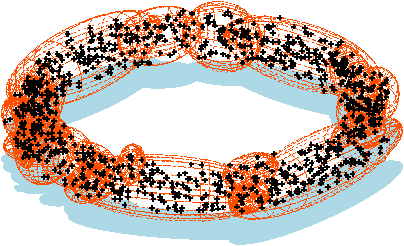
\includegraphics[width=\textwidth]{figures/multinest}
    %    \end{column} 
    %\end{columns}
    \cols[0.5]{%
        \texttt{MultiNest}
        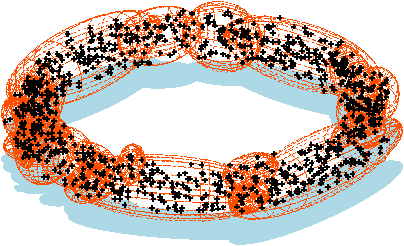
\includegraphics[width=0.8\textwidth]{figures/multinest}
            \vfill
        \texttt{DNest}
        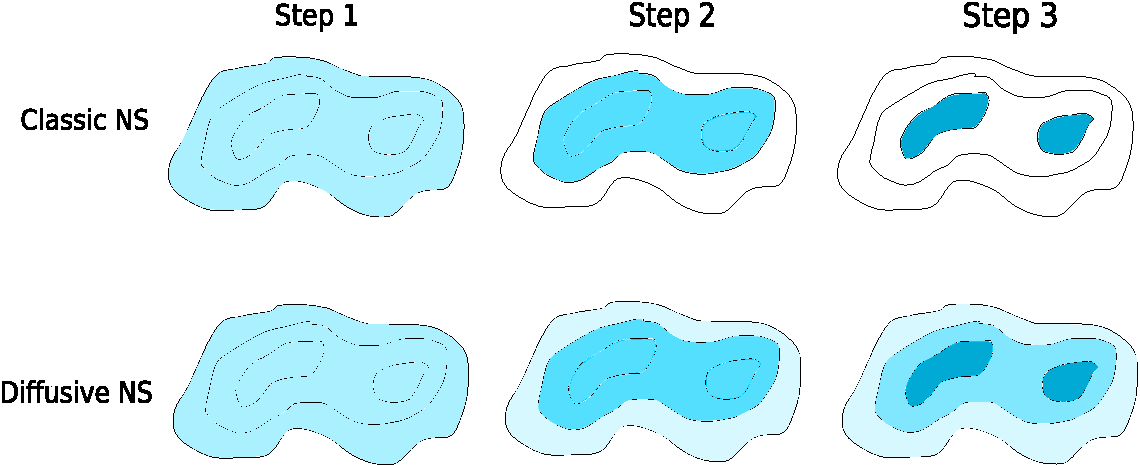
\includegraphics[width=\textwidth]{figures/dnest}
    }{%
        \texttt{PolyChord}
        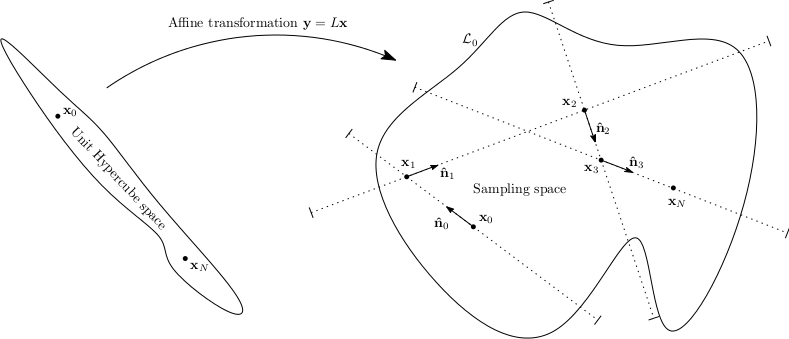
\includegraphics[width=\textwidth]{figures/polychord}
        \vfill
        \texttt{NeuralNest}
            \cols[0.5]{
                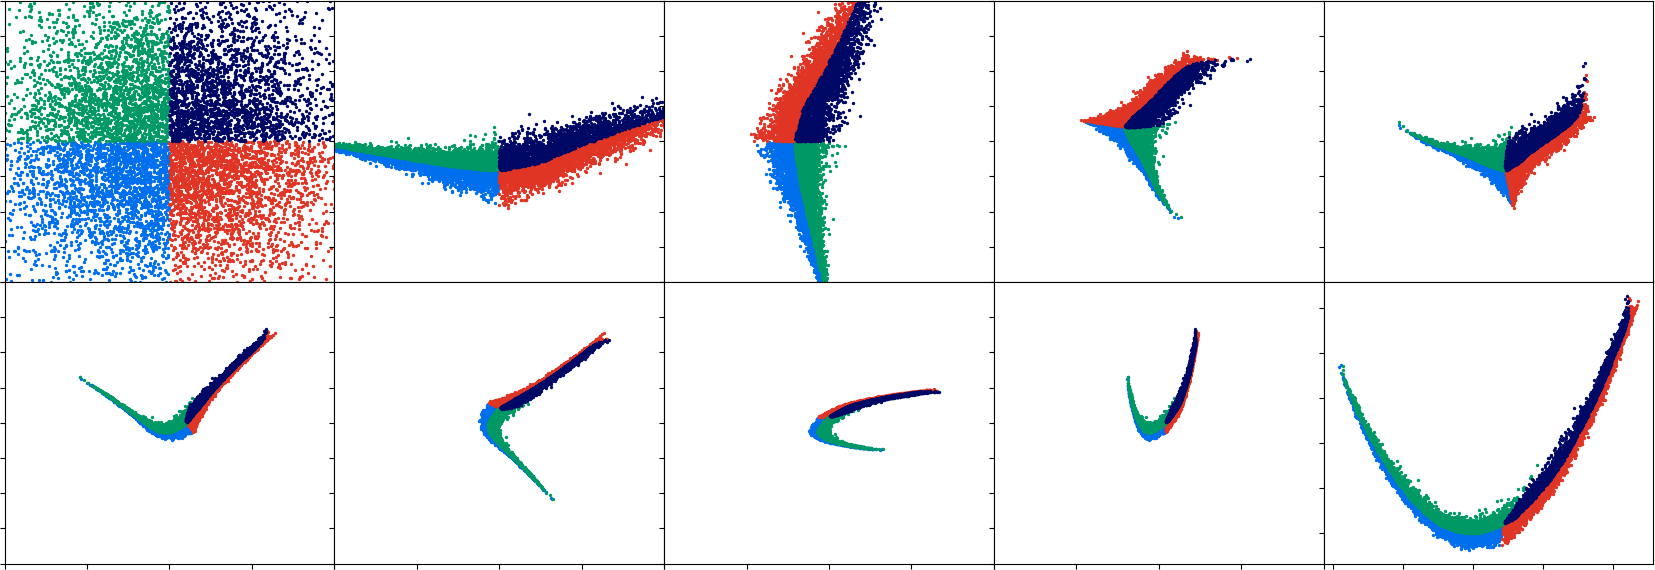
\includegraphics[width=\textwidth]{figures/rosenbrock_flow.png}
                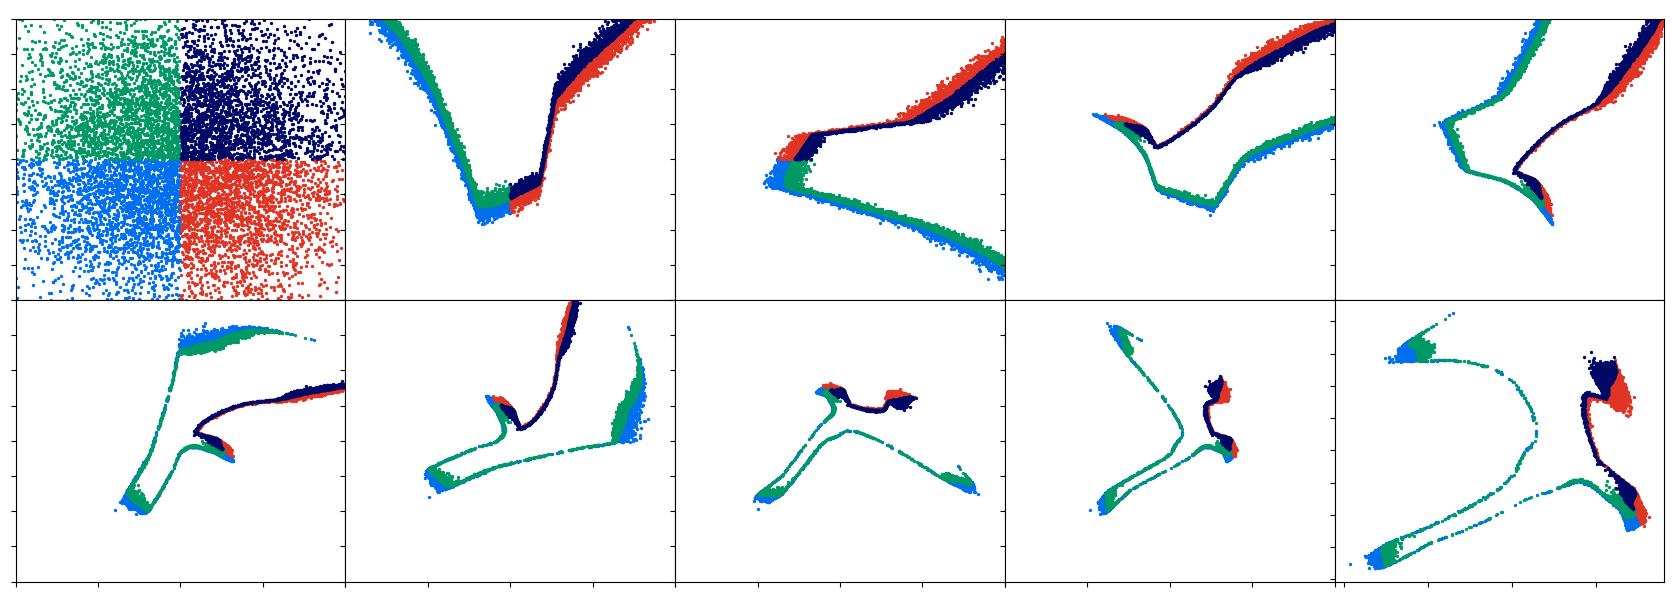
\includegraphics[width=\textwidth]{figures/himmelblau_flow.png}
            }{
                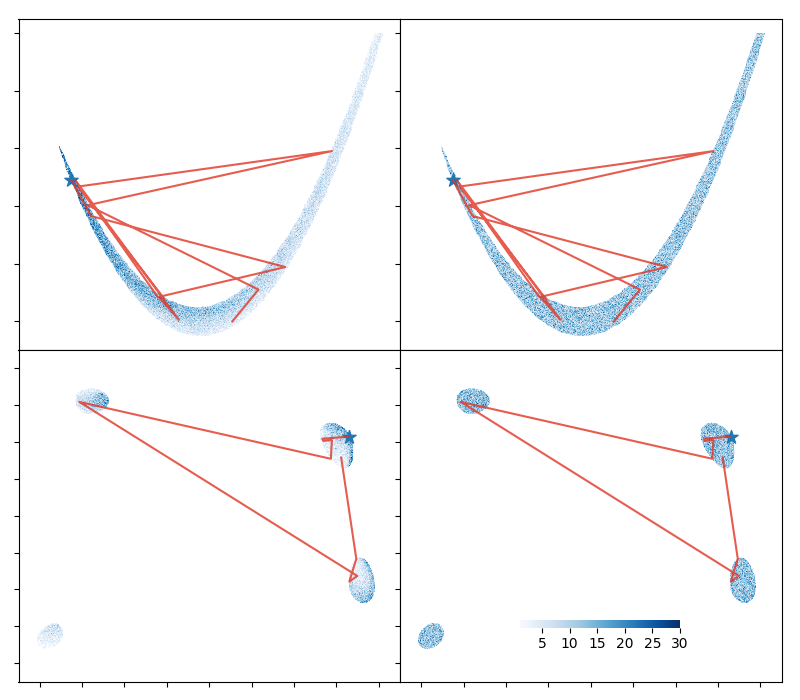
\includegraphics[width=\textwidth]{figures/chains.png}
            }
            \vfill
    }
\end{frame}

\begin{frame}
    \frametitle{Nested Sampling: Benefits and drawbacks}
    Relative to traditional numerical posterior samples (Metropolis Hastings, HMC, emcee), nested sampling:
    \begin{description}
        \item[$+$] Can calculate evidence (and therefore perform model comparison).
        \item[$+$] Can handle multi-modal distributions.
        \item[$+$] Requires little tuning for an a-priori unseen problem.
        \item[$+$] Highly parallelisable ($n_\mathrm{cores} \sim n_\mathrm{live} \gg 4$).
        \item[$-$] Slower than a well-tuned posterior sampler.
        \item[$-$] Run time is dependent on prior choice, and priors must be proper \\(some people view this as a feature rather than a bug).
    \end{description}
\end{frame}


\begin{frame}
    \frametitle{Nested Sampling: a user's guide}
    \begin{enumerate}
        \item Nested sampling is a likelihood scanner, rather than posterior explorer.
            \begin{itemize}
                \item This means typically most of its time is spent on burn-in rather than posterior sampling
                \item Changing the stopping criterion from $10^{-3}$ to $0.5$ does little to speed up the run, but can make results very unreliable
            \end{itemize}
        \item The number of live points $n_\mathrm{live}$ is a resolution parameter.
            \begin{itemize}
                \item Run time is linear in $n_\mathrm{live}$, posterior and evidence accuracy goes as $\frac{1}{\sqrt{n_\mathrm{live}}}$.
                \item Set low for exploratory runs $\sim\mathcal{O}(10)$ and increased to $\sim\mathcal{O}(1000)$ for production standard.
            \end{itemize}
        \item Most algorithms come with additional reliability parameter(s).
            \begin{itemize}
                \item e.g. \texttt{MultiNest}: $\text{eff}$, \texttt{PolyChord}: $n_\mathrm{repeats}$
                \item These are parameters which have no gain if set too conservatively, but increase the reliability
                \item Check that results do not degrade if you reduce them from defaults, otherwise increase.
            \end{itemize}
    \end{enumerate}
\end{frame}


\begin{frame}
    \frametitle{Key tools for Nested Sampling}
    \begin{description}
        \item[\texttt{anesthetic}] Nested sampling post processing \arxiv{1905.04768}\\
        \item[\texttt{insertion}] cross-checks using order statistics \arxiv{2006.03371}
            \hspace{5pt}\url{github.com/williamjameshandley/anesthetic}
        \item[\texttt{nestcheck}] cross-checks using unthreaded runs \arxiv{1804.06406}\\
            \hspace{5pt}\url{github.com/ejhigson/nestcheck}
        \item[\texttt{MultiNest}] Ellipsoidal rejection sampling \arxiv{0809.3437}\\
            \hspace{5pt}\url{github.com/farhanferoz/MultiNest}
        \item[\texttt{PolyChord}] Python/C++/Fortran state of the art \arxiv{1506.00171}\\
            \hspace{5pt}\url{github.com/PolyChord/PolyChordLite} 
        \item[\texttt{dynesty}] Python re-implementation of several codes \arxiv{1904.02180}\\
            \hspace{5pt}\url{github.com/joshspeagle/dynesty}
    \end{description}
\end{frame}


%\begin{frame}
%    \frametitle{Likelihood free inference}
%    <+Content+>
%\end{frame}

\begin{frame}
    \frametitle{FAQs}
    
    \begin{itemize}
    \item What was that awesome website? \\
    \hfill Full credit to Chi-feng for this incredible online demonstration tool\\
    \hfill \href{https://chi-feng.github.io/mcmc-demo/}{chi-feng.github.io/mcmc-demo/}

    \item How do you make your plots look hand-drawn? \\
        \hfill \texttt{import matplotlib.pyplot as plt; plt.xkcd()}
    \end{itemize}
\end{frame}



\end{document}
